\documentclass[a4paper,10pt]{report}
\usepackage[utf8]{inputenc}
\usepackage{graphicx}
\usepackage[francais]{babel}

% Title Page
\title{Annexes}
\author{Adrien DROGUET}


\begin{document}
\maketitle

\tableofcontents
\pagebreak

\chapter{Diagrammes de classe}

\section{core}
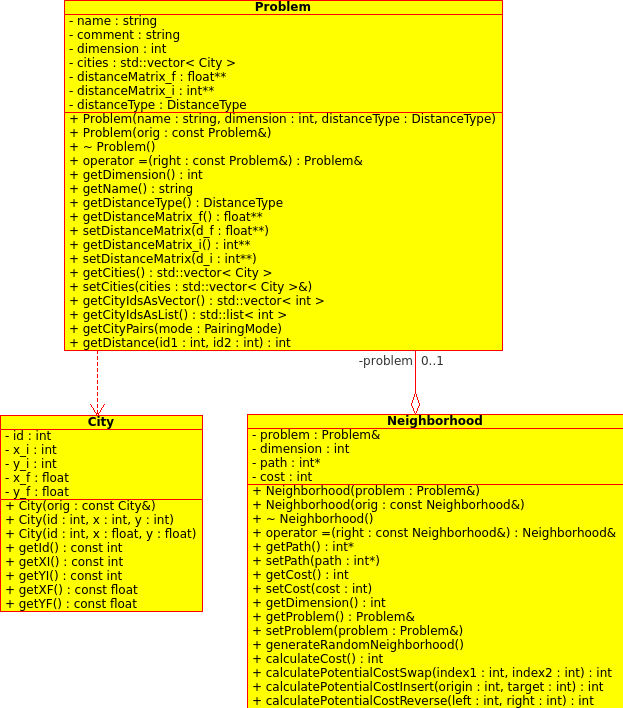
\includegraphics[width=\textwidth]{../UML/core.png}

\paragraph{}
\textbf{Problem} contient une matrice de distance, calculée une fois que toutes
les citées ont été enregistrées, qui va être l'attribut le plus important de
\textbf{Problem}, réutilisé par toutes les méthodes de calcul de coût.

\section{relation}
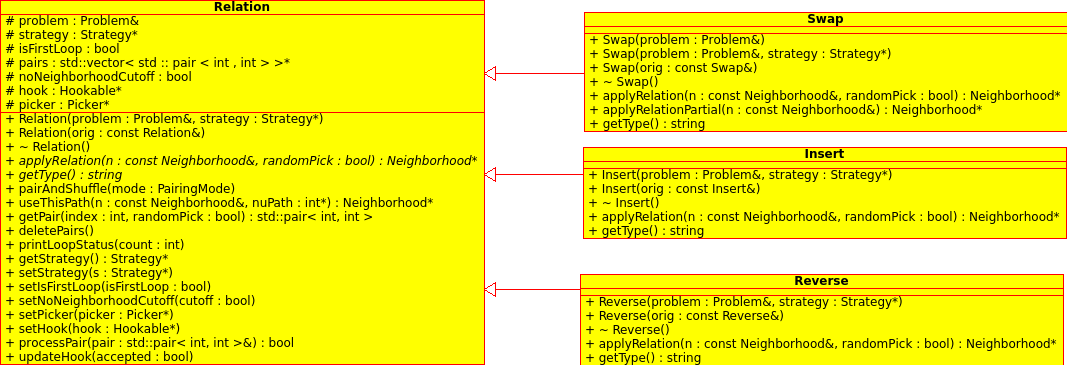
\includegraphics[width=\textwidth]{../UML/relation.png}

\section{strategy}
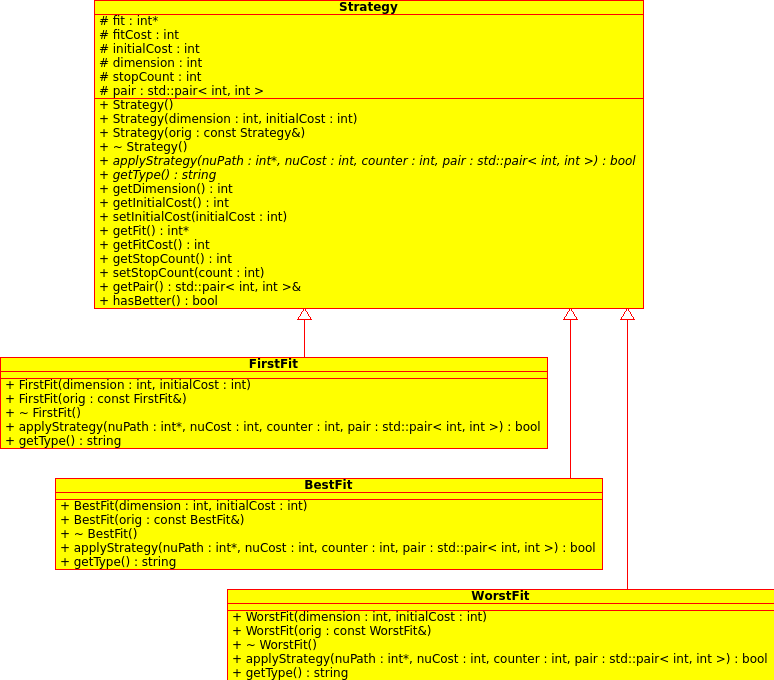
\includegraphics[width=\textwidth]{../UML/strategy.png}

\section{run}
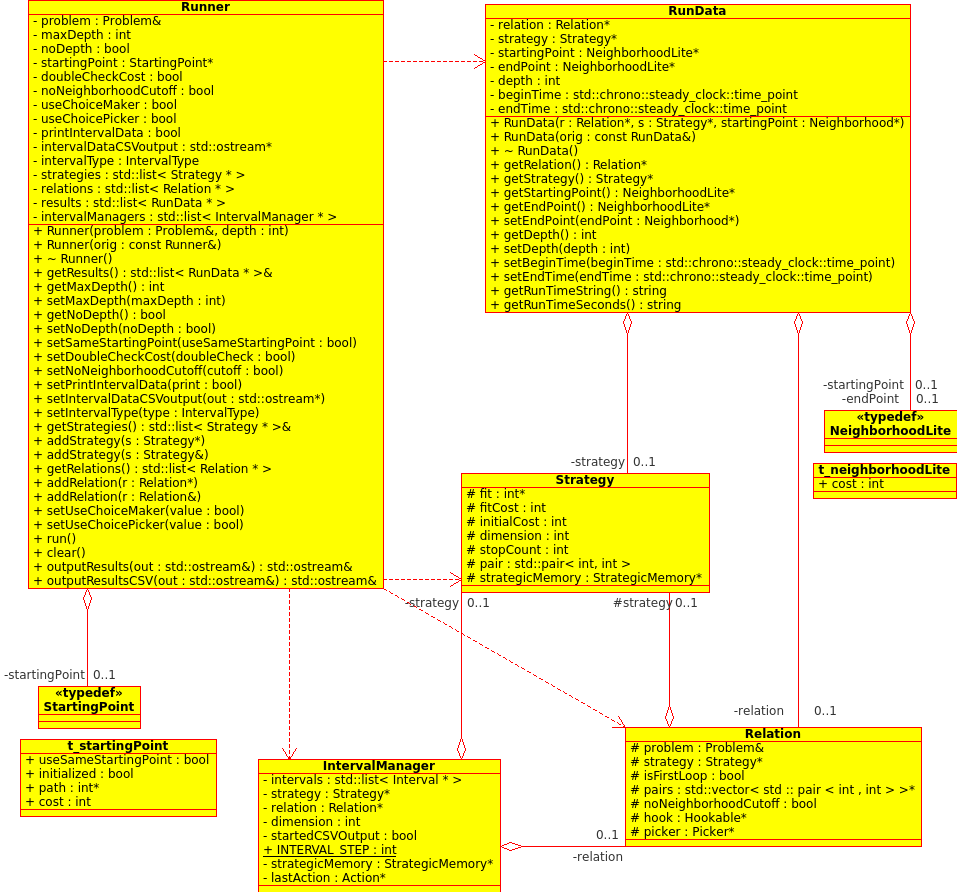
\includegraphics[width=\textwidth]{../UML/run.png}

\subsection{interval}
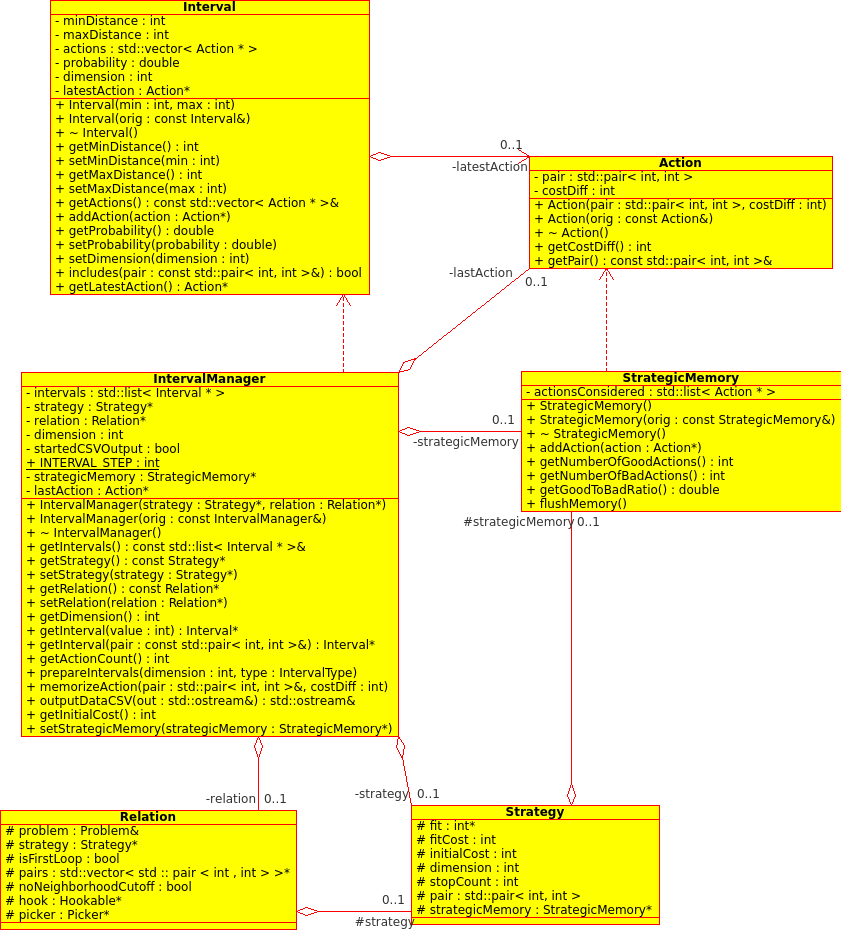
\includegraphics[width=\textwidth]{../UML/interval.png}

\section{hook}
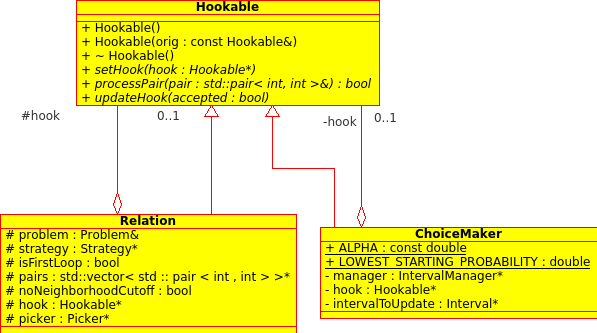
\includegraphics[width=\textwidth]{../UML/hook.png}

\section{choice}
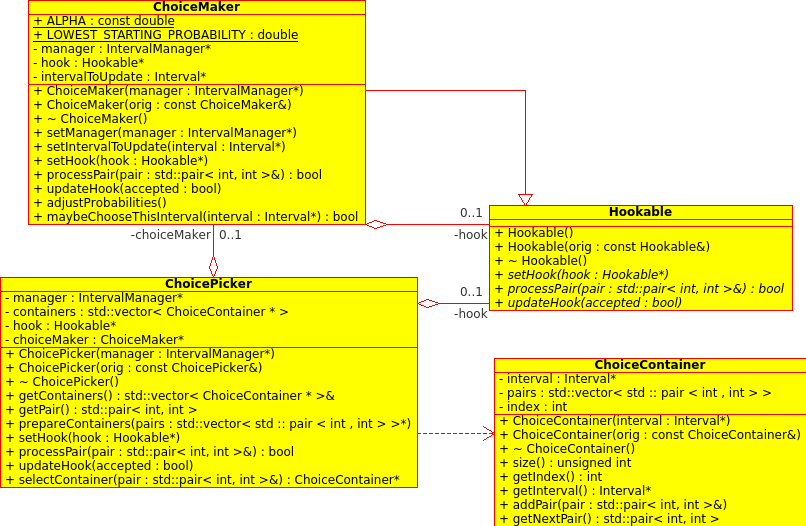
\includegraphics[width=\textwidth]{../UML/choice.png}

\chapter{Extraits de code}

\chapter{Résultats d'exécution}

\section{Résultats moyens}

\paragraph{}
  Les tableaux ci-dessous représente la compilation des résultats d'une
quarantaine d'exécutions.

\begin{figure}[h]
  \begin{center}
    \begin{tabular}{|l|r|r|r|}
      \hline
      &		\textbf{First Fit}&	\textbf{Best Fit}&	\textbf{Worst
Fit}\\\hline
      \textbf{Swap}&
	  6 012,195&
	  6 610,488&
	  6 007,561\\\hline
      \textbf{Insert}&
	  4 560,732&
	  4 804,634&
	  4 663,171\\\hline
      \textbf{Reverse}&
	  4 389,024&
	  4 388,293&
	  4 416,341\\\hline
    \end{tabular}
    \caption{Résultats moyens pour le TSP berlin52}
  \end{center}
\end{figure}

\begin{figure}[h]
  \begin{center}
    \begin{tabular}{|l|r|r|r|}
      \hline
      &		\textbf{First Fit}&	\textbf{Best Fit}&	\textbf{Worst
Fit}\\\hline
      \textbf{Swap}&
	  204 979,051&
	  216 486,103&
	  198 029,436\\\hline
      \textbf{Insert}&
	  168 662,564&
	  174 234,641&
	  169 584,231\\\hline
      \textbf{Reverse}&
	  154 457,282&
	  151 268,590&
	  158 711,872\\\hline
    \end{tabular}
    \caption{Résultats moyens pour le TSP bier127}
  \end{center}
\end{figure}

\begin{figure}[h]
  \begin{center}
    \begin{tabular}{|l|r|r|r|}
      \hline
      &		\textbf{First Fit}&	\textbf{Best Fit}&	\textbf{Worst
Fit}\\\hline
      \textbf{Swap}&
	  6 367,200&
	  6 989,250&
	  5 497,750\\\hline
      \textbf{Insert}&
	  3 647,000&
	  4 368,950&
	  3 484,050\\\hline
      \textbf{Reverse}&
	  2 855,500&
	  2 856,250&
	  2 859,800\\\hline
    \end{tabular}
    \caption{Résultats moyens pour le TSP ch130}
  \end{center}
\end{figure}

\begin{figure}[h]
  \begin{center}
    \begin{tabular}{|l|r|r|r|}
      \hline
      &		\textbf{First Fit}&	\textbf{Best Fit}&	\textbf{Worst
Fit}\\\hline
      \textbf{Swap}&
	  7 774,650&
	  7 876,250&
	  5 949,600\\\hline
      \textbf{Insert}&
	  4 253,050&
	  5 281,000&
	  3 752,950\\\hline
      \textbf{Reverse}&
	  3 257,550&
	  3 257,200&
	  3 264,750\\\hline
    \end{tabular}
    \caption{Résultats moyens pour le TSP ch150}
  \end{center}
\end{figure}

\section{interval sheets}

%screens + description

\end{document}          
